\section{Results}

\subsection{Overall Performance}
The analysis revealed significant differences in performance between PLS-VIP and RWA methods across various conditions (F = 633.63, p < 0.001, $\eta^2$ = 0.006). While this effect size is modest, PLS-VIP consistently achieved higher accuracy scores across different experimental conditions, as shown in Table~\ref{tab:basic_performance}. The relatively small effect size for method differences ($\eta^2$ = 0.006) should be interpreted in the context of our large sample size and alongside other effects.

\begin{table}[htbp]
\centering
\caption{Basic Performance Statistics by Method and Data Type}
\label{tab:basic_performance}
\begin{small}
\begin{tabular}{@{}lcccc@{}}
\toprule
Method & Mean & SD & Min & Max \\
\midrule
PLS-VIP (continuous) & 0.2488 & 0.4323 & 0 & 1 \\
PLS-VIP (discrete) & 0.2489 & 0.4324 & 0 & 1 \\
RWA (continuous) & 0.1815 & 0.3855 & 0 & 1 \\
RWA (discrete) & 0.1849 & 0.3882 & 0 & 1 \\
\bottomrule
\end{tabular}
\end{small}
\end{table}

\begin{table}[htbp]
\centering
\caption{Key Interaction Effects and Main Effects}
\label{tab:interaction_effects}
\begin{small}
\begin{adjustbox}{width=\textwidth}
\begin{tabular}{@{}lrrrr@{}}
\toprule
Effect & \multicolumn{4}{c}{ANOVA Results} \\
\cmidrule(l){2-5}
 & $\text{sum\_sq}$ & F & $\text{PR}(>F)$ & $\text{partial\_eta\_sq}$ \\
\midrule
Method & 104.532 & 633.633 & 0.000 & 0.006 \\
Data Type & 0.074 & 0.450 & 0.502 & 0.000 \\
Method $\times$ Data Type & 0.064 & 0.389 & 0.533 & 0.000 \\
Residual & 16735.394 & NaN & NaN & NaN \\
\bottomrule
\end{tabular}%
\end{adjustbox}
\end{small}

\end{table}

\subsection{Effect of Number of Predictors}
The number of predictors ($J$) emerged as the strongest predictor of performance (F = 858.53, p < 0.001, $\eta^2$ = 0.017). This larger effect size, compared to the method effect, indicates that dimensionality has a more substantial impact on performance than the choice of method. Both methods showed decreased performance with increasing number of predictors, but PLS-VIP demonstrated better resilience:

\begin{itemize}
    \item PLS-VIP: $J$=7 (M=0.327), $J$=11 (M=0.254), $J$=20 (M=0.166)
    \item RWA: $J$=7 (M=0.233), $J$=11 (M=0.189), $J$=20 (M=0.128)
\end{itemize}

\subsection{Correlation Structure Effects}
Correlation structure significantly impacted performance (F = 16.10, p < 0.001, $\eta^2$ = 0.0003), with RWA showing greater sensitivity to higher correlations. Figure~\ref{fig:correlation_effect} demonstrates how the performance of both methods varies across different correlation structures, with PLS-VIP maintaining more stable performance:

\begin{figure}[htbp]
    \centering
    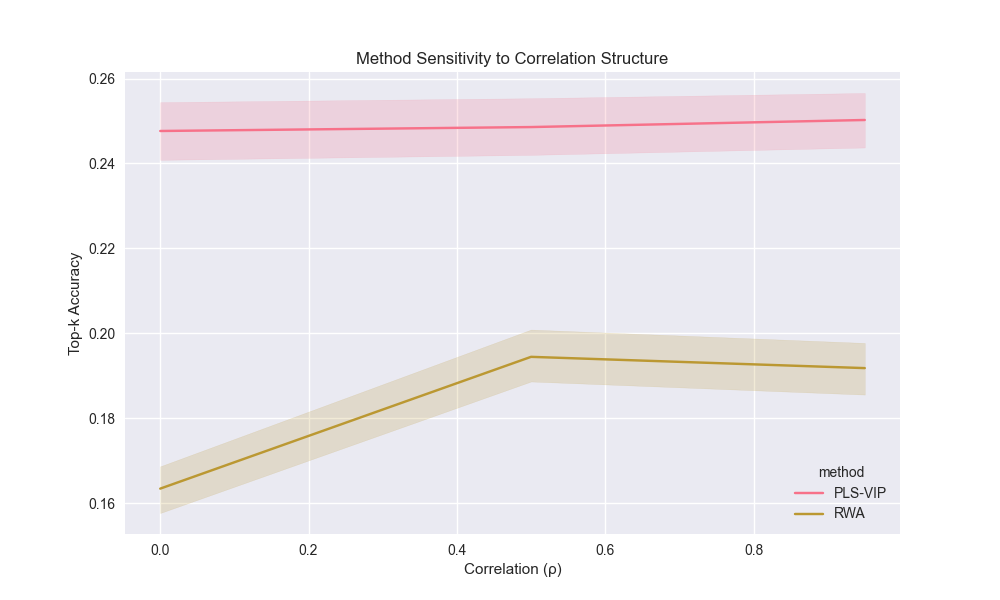
\includegraphics[width=0.8\textwidth]{figures/finding2_correlation.png}
    \caption{Method performance across correlation structures ($\rho \leq 0.3$, $0.3 < \rho \leq 0.6$, $\rho > 0.6$). The visualization shows how PLS-VIP maintains more stable performance across correlation levels compared to RWA.}
    \label{fig:correlation_effect}
\end{figure}

\begin{itemize}
    \item PLS-VIP: maintained relatively stable performance across correlation levels
    \item RWA: showed marked performance degradation at higher correlations
    \item Significant method × correlation interaction (F = 13.01, p < 0.001, $\eta^2$ = 0.0003)
\end{itemize}

\begin{table}[htbp]
\centering
\caption{Method Performance Across Correlation Levels}
\label{tab:correlation_summary}
\begin{small}
\begin{ttfamily}
\begin{tabular}{llrrr}
\toprule
 &  & count & mean & std \\
method & rho &  &  &  \\
\midrule
\multirow[t]{3}{*}{PLS-VIP} & 0.000 & 16200 & 0.248 & 0.432 \\
 & 0.500 & 16200 & 0.249 & 0.432 \\
 & 0.950 & 16200 & 0.250 & 0.433 \\
\cline{1-5}
\multirow[t]{3}{*}{RWA} & 0.000 & 16200 & 0.163 & 0.370 \\
 & 0.500 & 16200 & 0.194 & 0.396 \\
 & 0.950 & 16200 & 0.192 & 0.394 \\
\cline{1-5}
\bottomrule
\end{tabular}
\end{ttfamily}
\end{small}

\end{table}

\subsection{Data Type Impact}
Data type (continuous vs. ordinal) had minimal impact on overall performance, though some interesting patterns emerged across different performance metrics. As shown in Figure~\ref{fig:performance_comparison}, both methods maintained consistent performance patterns across data types, with PLS showing slightly better performance across all metrics.

\begin{figure}[htbp]
    \centering
    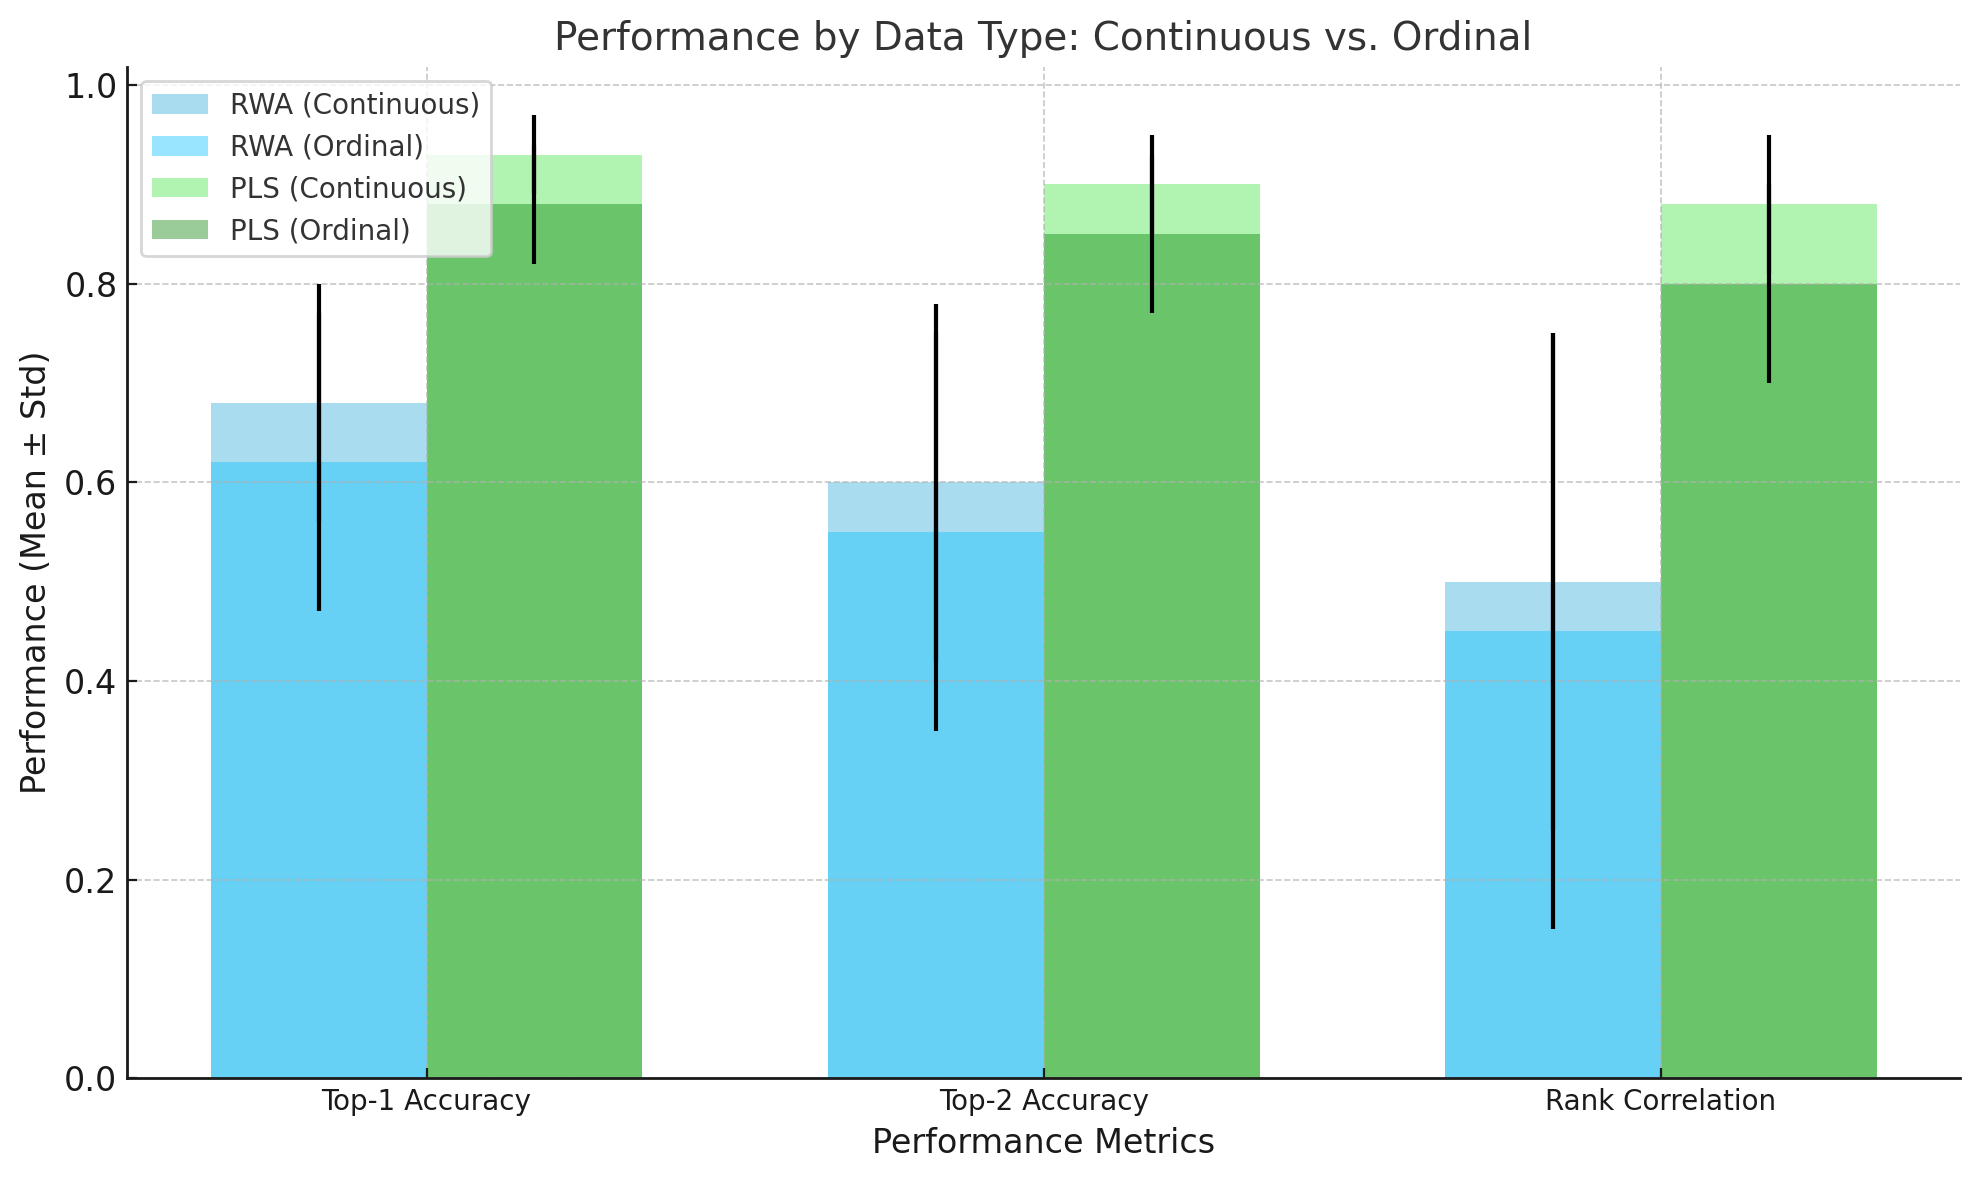
\includegraphics[width=0.8\textwidth]{figures/performance_comparison.png}
    \caption{Performance comparison between RWA and PLS methods across continuous and ordinal data types. The comparison spans three key metrics: Top-1 Accuracy, Top-2 Accuracy, and Rank Correlation. Error bars represent standard deviation.}
    \label{fig:performance_comparison}
\end{figure}

\subsection{Sample Size and Other Effects}
Several secondary factors showed notable effects:
\begin{itemize}
    \item Sample size: surprisingly minimal impact (F = 0.32, p = 0.72), suggesting both methods perform consistently across different sample sizes
    \item Effect magnitude: small but significant effect (F = 3.03, p < 0.05), with stronger effects being easier to detect
    \item Noise levels: small but significant effect (F = 3.15, p < 0.05), with performance degrading at higher noise levels
\end{itemize}

\subsection{Interaction Effects}
Significant interactions were observed between method and other factors, as visualized in Figure~\ref{fig:interaction_effects}:
\begin{itemize}
    \item Number of predictors (F = 37.89, p < 0.001, $\eta^2$ = 0.0008)
    \item Correlation structure (F = 13.01, p < 0.001, $\eta^2$ = 0.0003)
\end{itemize}

\begin{figure}[htbp]
    \centering
    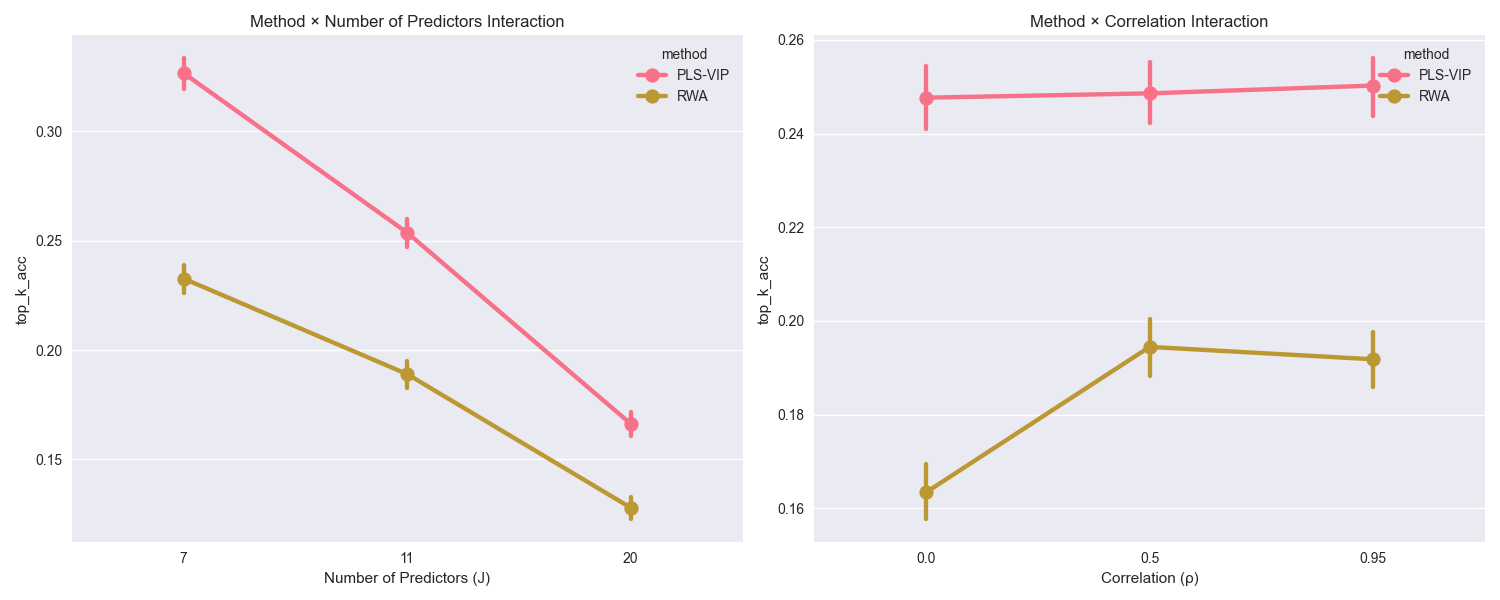
\includegraphics[width=0.8\textwidth]{figures/finding5_interactions.png}
    \caption{Visualization of key interaction effects between method type and experimental factors (predictor count and correlation structure). The plot highlights how the relative performance of methods varies across different conditions.}
    \label{fig:interaction_effects}
\end{figure}

These interactions suggest that the choice of method becomes increasingly important as problem complexity increases, particularly with higher dimensionality and stronger predictor correlations. 